%CHAPTER
\chapter{Uživatelská dokumentace}  \label{chap:uziv_doc}
Pro instalaci celého úložiště je potřeba mít nainstalovanou aplikaci \textbf{Docker}.

\section{Adresářová struktura}
Adresářová struktura je následující:
\begin{itemize}
\item \textbf{Aplikace\_a\_knihovny}
	\begin{itemize}
	\item \textbf{docker}
		\begin{itemize}
		\item \textbf{init} - Inicializační skripty pro MySQL, MongoDB a Apache Kafka.
		\item \textbf{mongo\_import} - Soubory pro import dat do MongoDB.
		\item \textbf{docker-compose.yml}
		\item \textbf{Dockerfile}
		\end{itemize}
	\end{itemize}
\item \textbf{Poster}
\item \textbf{Text\_prace}
\item \textbf{Vstupni\_data}
	\begin{itemize}
	\item \textbf{mongodb}
		\begin{itemize}
		\item \textbf{patents} - Složka se soubory obsahující patentová data.
		\end{itemize}
	\item \textbf{mysql}
		\begin{itemize}
		\item \textbf{patents.sql} - SQL soubor s patentovými daty.
		\end{itemize}
	\end{itemize}
\item \textbf{Readme.txt}
\end{itemize}
\newpage
\section{Instalace úložiště}
Instalace úložiště a všech potřebných aplikací se provádí následovně:
\begin{enumerate}
\item Otevřít konzoli ve složce \textbf{./Aplikace\_a\_knihovny/docker}.
\item Spustit příkaz \textbf{docker-compose up}. Docker začne stahovat všechny aplikace (jejich image), následně pro ně vytvoří kontejnery, které poté spustí (viz obrázky č. \ref{fig:docker_compose}, \ref{fig:docker_containers}).
	\begin{figure}[H]
	\centering
	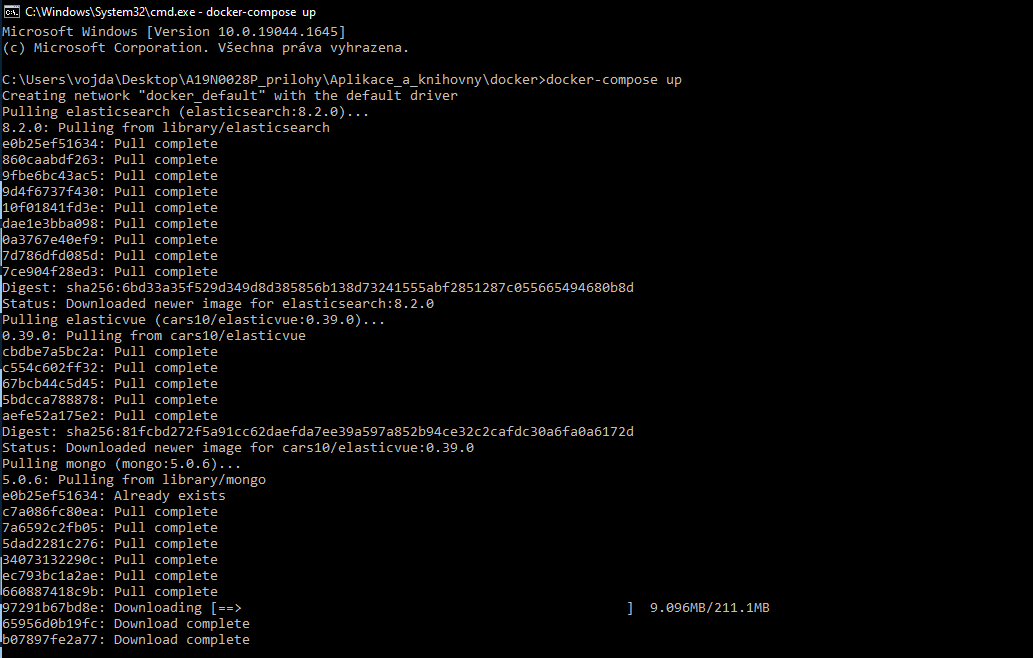
\includegraphics[width=16cm]{img/manual/docker_compose}
	\caption{Docker compose a stahování aplikací.}
	\label{fig:docker_compose}
	\end{figure}
		\begin{figure}[H]
	\centering
	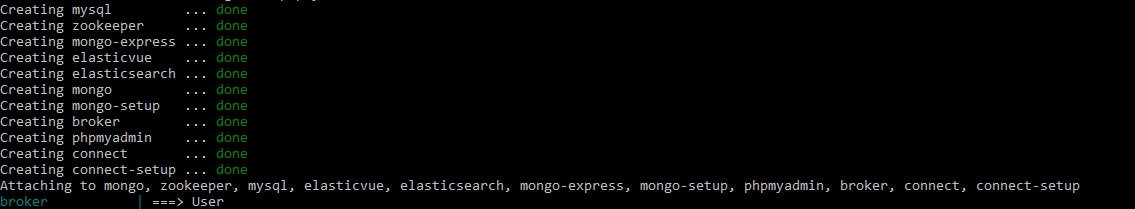
\includegraphics[width=16cm]{img/manual/docker_create_containers}
	\caption{Vytvoření kontejnerů v dockeru.}
	\label{fig:docker_containers}
	\end{figure}
\item Veškerá instalace a nastavování končí ve chvíli, kdy konektor mezi MongoDB a Apache Kafka začne posílat zprávy (viz obrázek č. \ref{fig:docker_done_creating}).
		\begin{figure}[H]
	\centering
	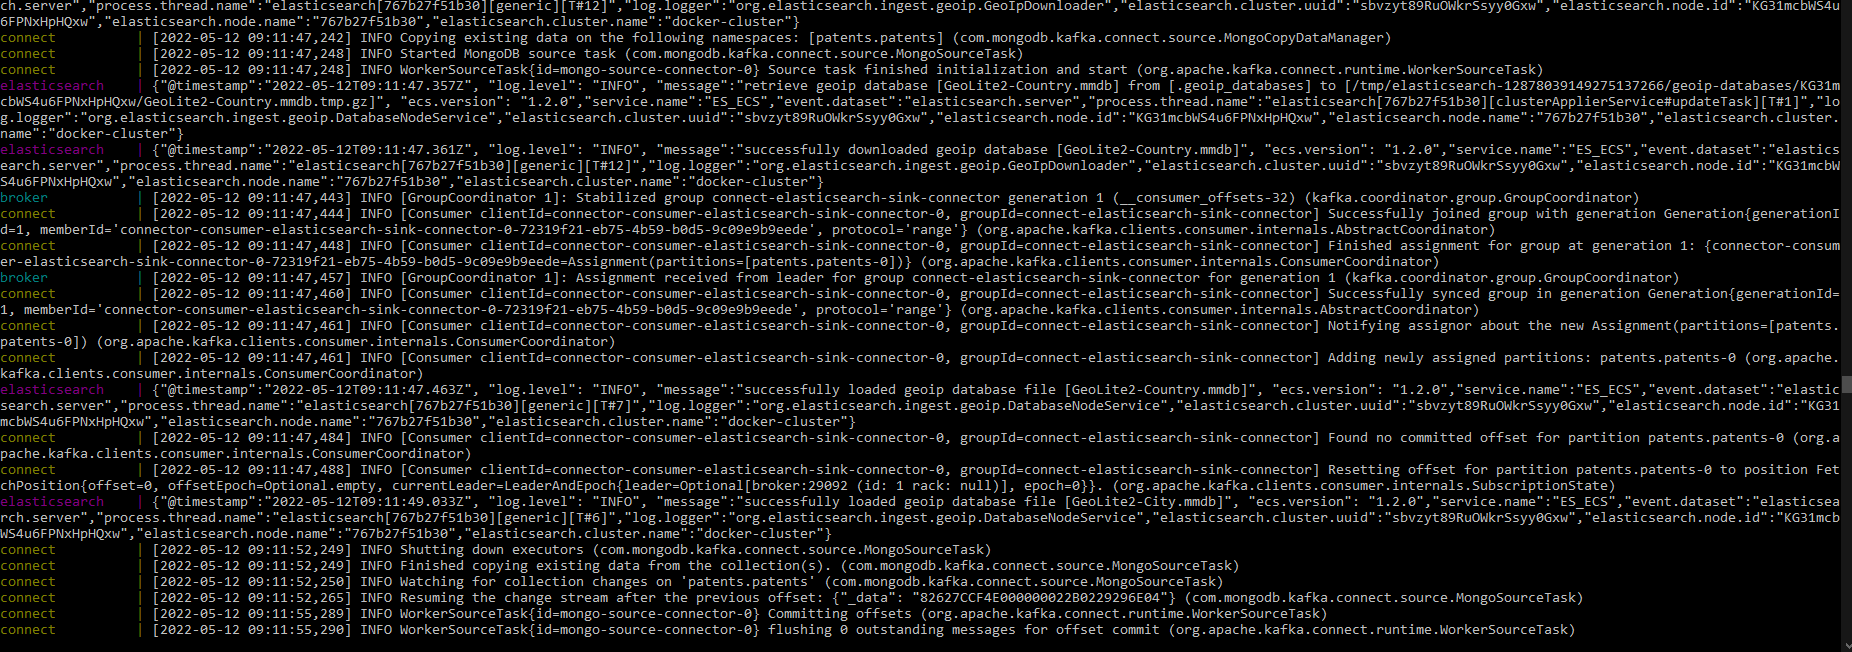
\includegraphics[width=16cm]{img/manual/docker_done_creating}
	\caption{Úspěšná instalace a nastavení všech aplikací.}
	\label{fig:docker_done_creating}
	\end{figure}
\end{enumerate}

\subsection{Smazání setup kontejnerů}
Nastavovací moduly slouží pouze pro prvotní nastavení MongoDB a Apache Kafka Connect, takže po jejich úspěšném vykonání je lze smazat. Smazání se provede následujícím způsobem (ukázka na obrázku č. \ref{fig:docker_remove}):
\begin{enumerate}
\item Kdekoliv v systému otevřít konzoli a zadat příkaz \textbf{docker container ls -a}, pomocí kterého zjistíme všechny existující kontejnery v dockeru.
\item Zjistíme ID kontejneru pro oba nastavovací moduly. Jména nastavovacích modulů jsou \textbf{connect-setup} a \textbf{mongo-setup}.
\item Zadáme příkaz \textbf{docker rm CONTAINER\_ID}, kde \textit{CONTAINER\_ID} je ID kontejneru nastavovacího modulu.
\end{enumerate}
	\begin{figure}[H]
	\centering
	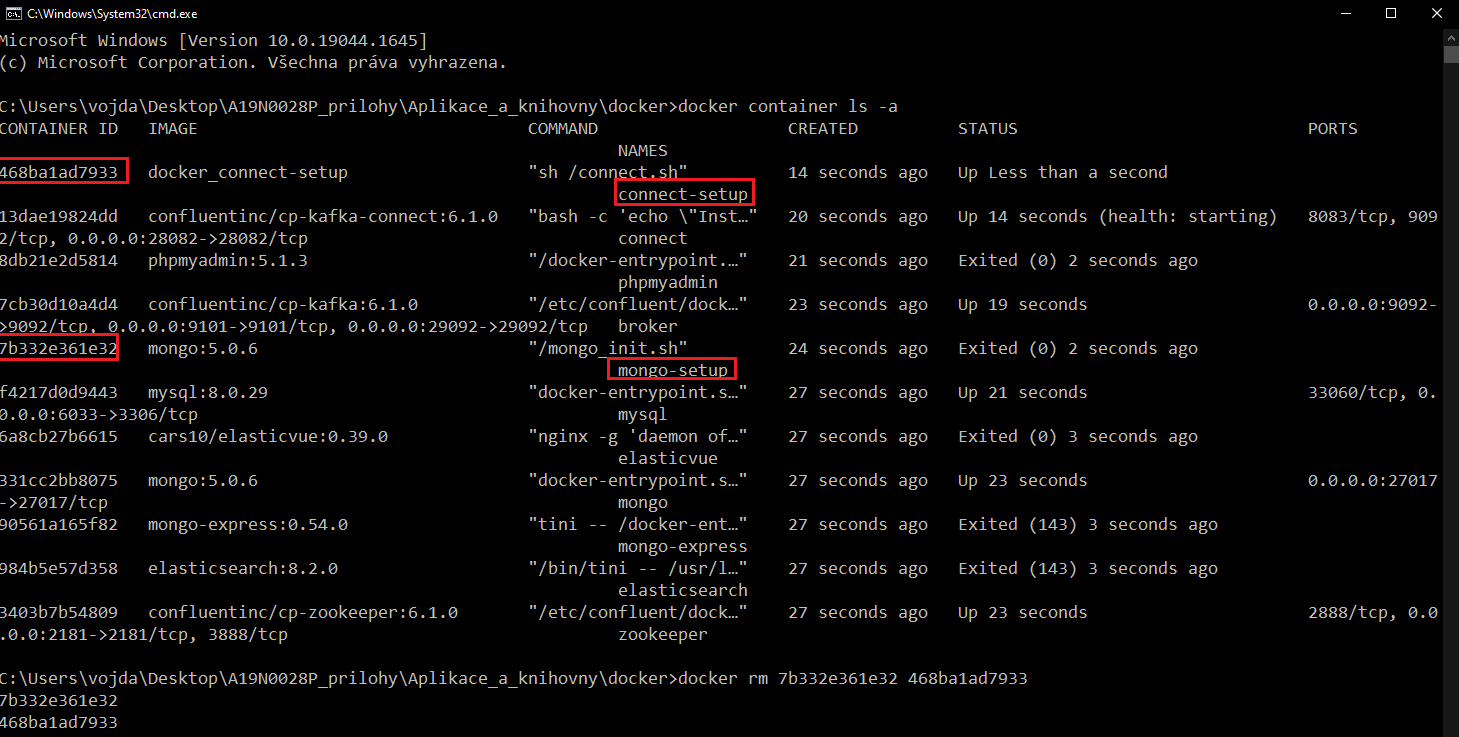
\includegraphics[width=16cm]{img/manual/docker_remove}
	\caption{Smazání kontejnerů pro nastavovací moduly.}
	\label{fig:docker_remove}
	\end{figure}

\newpage
\section{Import dat do MySQL}
Import dat se provádí pomocí PHPMyAdmin na adrese \textbf{http://localhost:8082/}. Postup pro import je následující:
\begin{enumerate}
\item Ve webovém prohlížeči otevřít stránku \textbf{http://localhost:8082/}.
\item Přihlásit se s následujícími údaji: \textbf{Jméno}: \textit{root}, \textbf{Heslo}: \textit{password} (viz obrázek č. \ref{fig:mysqllogin})
	\begin{figure}[H]
	\centering
	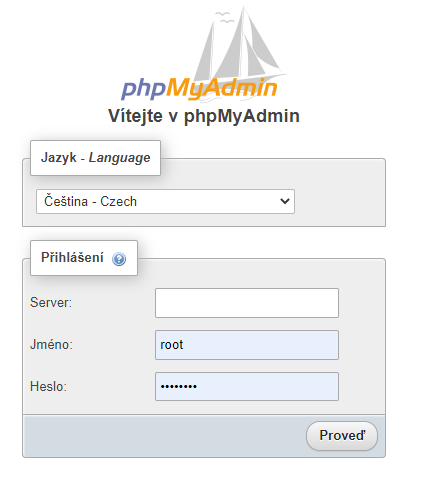
\includegraphics[width=10cm]{img/manual/mysql_login}
	\caption{PHPMyAdmin přihlášení.}
	\label{fig:mysqllogin}
	\end{figure}
\item Po přihlášení kliknout na databázi \textbf{patents} (viz obrázek č. \ref{fig:phpmyadmin}).
	\begin{figure}[H]
	\centering
	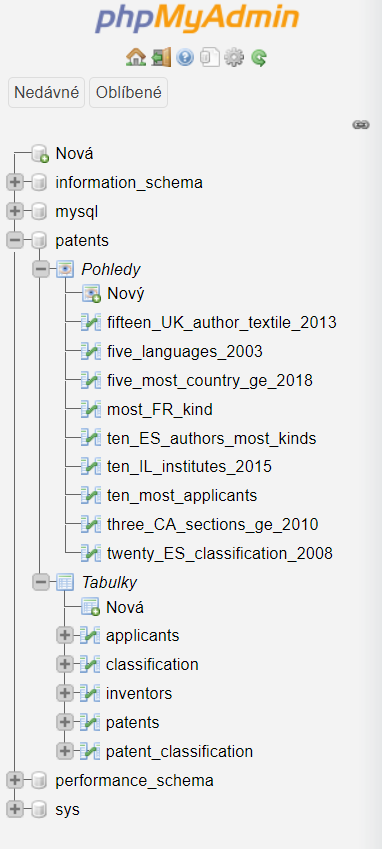
\includegraphics[width=8cm]{img/manual/phpmyadmin}
	\caption{Databáze v PHPMyAdmin.}
	\label{fig:phpmyadmin}
	\end{figure}
\item Na horní liště kliknout na záložku \textbf{Import}.
\item Kliknout na tlačítko \textbf{Vybrat soubor} a zvolit soubor \newline \textit{./Vstupni\_data/mysql/patents.sql} (viz obrázek č. \ref{fig:mysqlimport}).
	\begin{figure}[H]
	\centering
	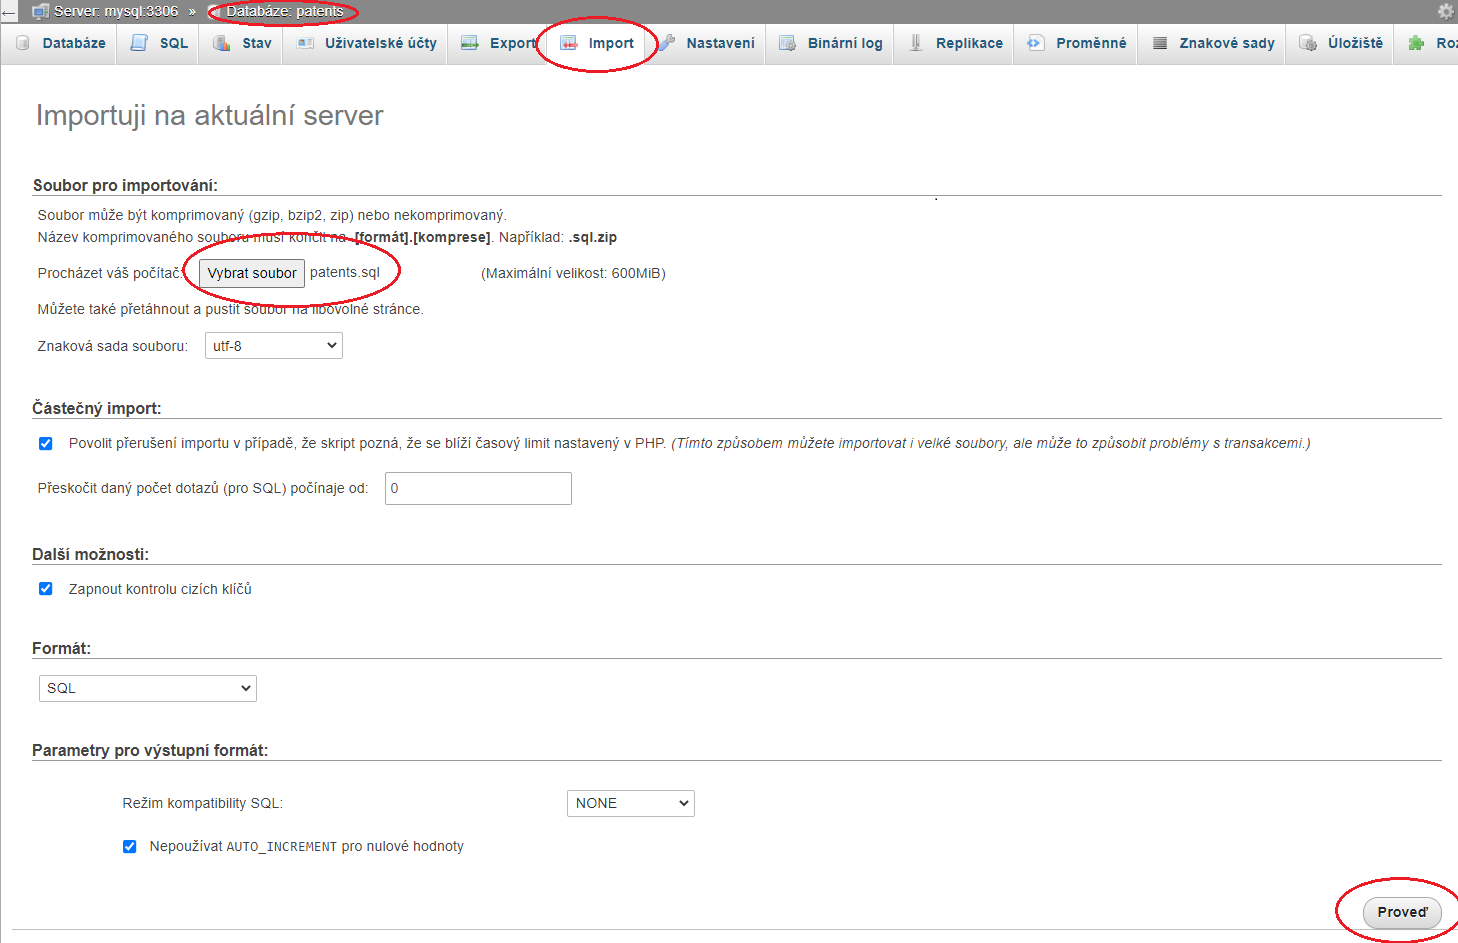
\includegraphics[width=14cm]{img/manual/mysql_import}
	\caption{Import dat v PHPMyAdmin.}
	\label{fig:mysqlimport}
	\end{figure}
\item Kliknout na tlačítko \textbf{Proveď} a počkat, než se naimportují všechna data do všech tabulek.
\item Po úspěšném importu dat se zobrazí hláška (viz obrázek č. \ref{fig:mysql_import_ok}).
	\begin{figure}[H]
	\centering
	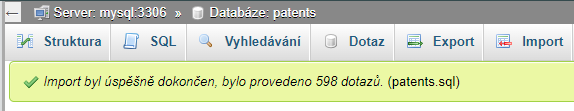
\includegraphics[width=12cm]{img/manual/mysql_import_ok}
	\caption{Úspěšný import dat v PHPMyAdmin.}
	\label{fig:mysql_import_ok}
	\end{figure}
\end{enumerate}

\newpage
\section{Import dat do MongoDB}
\todo{Ukázku výsledků z elasticu}
Import dat pro MongoDB se provádí pomocí oficiální aplikace od MongoDB s názvem \textbf{mongo\_restore.exe}. Postup pro import je následující:
\begin{enumerate}
\item Otevřít konzoli ve složce \textbf{./Aplikace\_a\_knihovny/docker/mongo\_import}.
\item Spustit dávkový soubor \textbf{import.bat} a počkat na import dat (viz obrázek č. \ref{fig:mongo_import}).
	\begin{figure}[H]
	\centering
	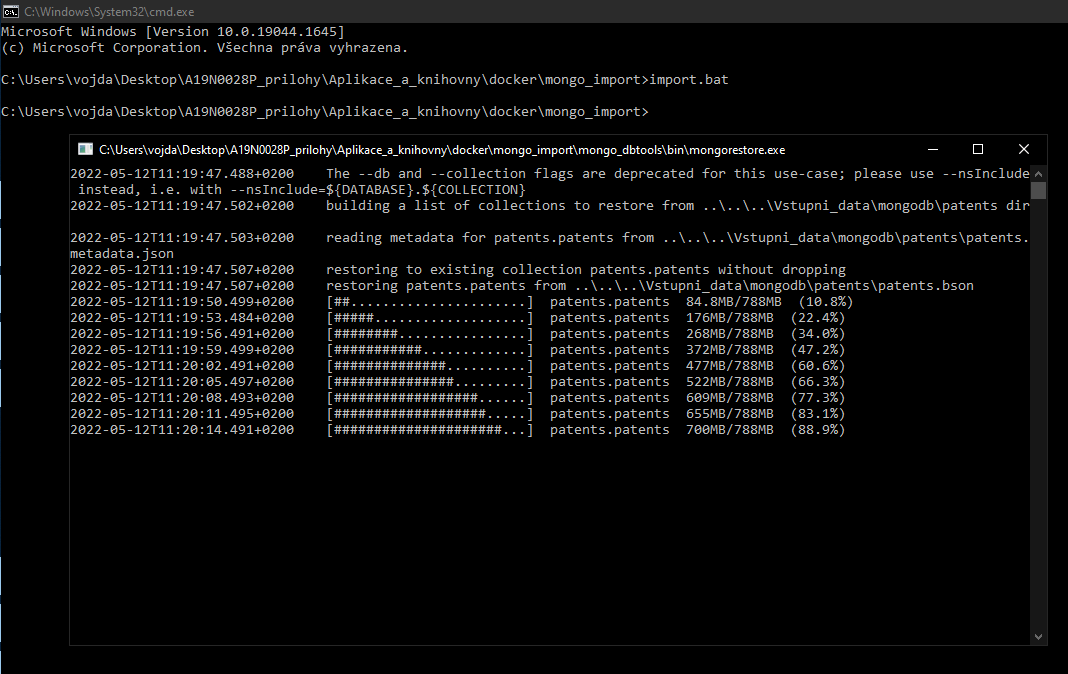
\includegraphics[width=14cm]{img/manual/mongo_import}
	\caption{Import dat do MongoDB.}
	\label{fig:mongo_import}
	\end{figure}
	\begin{itemize}
	\item Zároveň bude probíhat i import dat do Elasticsearch. Import dat do elasticu lze pozorovat v konzoli kde jsou spuštěné naše docker kontejnery (viz obrázek č. \ref{fig:elastic_import}). Apache Kafka vypisuje warning hlášky že se nepodařilo vykonat bulk request kvůli \newline\textit{java.lang.NullPointerException}. Toho se není potřeba obávat, protože to je pouze bug v rámci Apache Kafka Connect, který pouze vypisuje tyto hlášky, ale samotný import do Elasticsearch funguje.
		\begin{figure}[H]
		\centering
		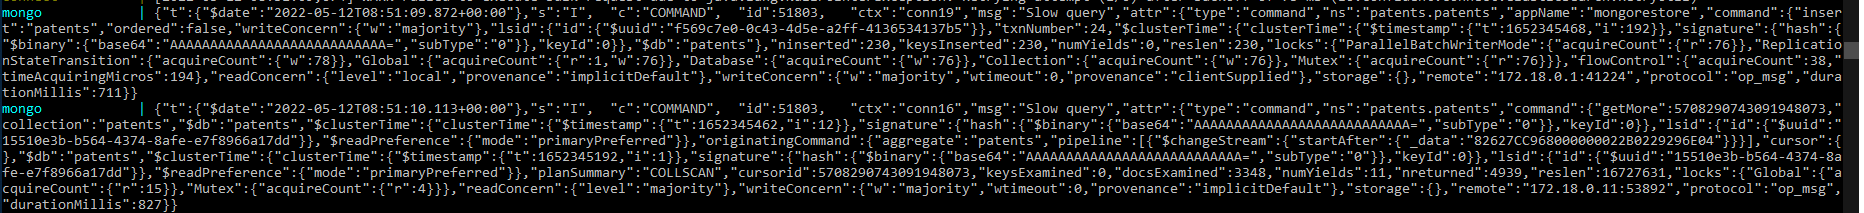
\includegraphics[width=14cm]{img/manual/mongo_import_console}
		\caption{Import dat do Elasticsearch.}
		\label{fig:elastic_import}
		\end{figure}
	\end{itemize}
\item Data do MongoDB jsou importována, lze provést kontrolu na adrese \textbf{http://localhost:8081/} v databázi \textbf{patents} a kolekci \textbf{patents} (viz obrázek č. \ref{fig:mongo_done_import}).
		\begin{figure}[H]
		\centering
		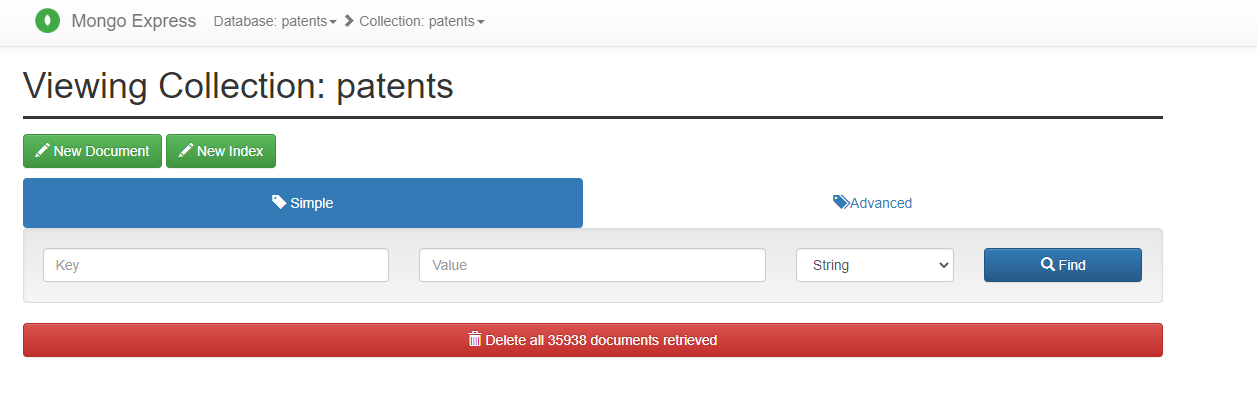
\includegraphics[width=15cm]{img/manual/mongo_import_done}
		\caption{Importovaná data v Mongo-express.}
		\label{fig:mongo_done_import}
		\end{figure}
\end{enumerate}